% -----------------------------------------------
% Template for ISMIR Papers
% 2018 version, based on previous ISMIR templates

% Requirements :
% * 6+n page length maximum
% * 4MB maximum file size
% * Copyright note must appear in the bottom left corner of first page
% * Clearer statement about citing own work in anonymized submission
% (see conference website for additional details)
% -----------------------------------------------

\documentclass{article}
\usepackage{ismir,amsmath,cite,url}
\usepackage{graphicx}
\usepackage{color}
\usepackage{xspace}
\usepackage{siunitx}
\usepackage{caption}
\usepackage{subcaption}
\usepackage{float}

\urlstyle{same}


\newcommand{\ml}[1]{\textcolor{blue}{ML : #1}}
\newcommand{\vl}[1]{\textcolor{red}{VL : #1}}

% Title.
% ------
\title{Extended playing techniques: \\
the next milestone in musical instrument recognition}

% Note: Please do NOT use \thanks or a \footnote in any of the author markup

% Three addresses
% --------------
\threeauthors
  {First Author} {Affiliation1 \\ {\tt author1@ismir.edu}}
  {Second Author} {\bf Retain these fake authors in\\\bf submission to preserve the formatting}
  {Third Author} {Affiliation3 \\ {\tt author3@ismir.edu}}

%% To make customize author list in Creative Common license, uncomment and customize the next line
%  \def\authorname{First Author, Second Author, Third Author}

% Four or more addresses
% OR alternative format for large number of co-authors
% ------------
%\multauthor
%{First author$^1$ \hspace{1cm} Second author$^1$ \hspace{1cm} Third author$^2$} { \bfseries{Fourth author$^3$ \hspace{1cm} Fifth author$^2$ \hspace{1cm} Sixth author$^1$}\\
%  $^1$ Department of Computer Science, University , Country\\
%$^2$ International Laboratories, City, Country\\
%$^3$  Company, Address\\
%{\tt\small CorrespondenceAuthor@ismir.edu, PossibleOtherAuthor@ismir.edu}
%}
%\def\authorname{First author, Second author, Third author, Fourth author, Fifth author, Sixth author}


%\sloppy % please retain sloppy command for improved formatting % how about no?

\hyphenation{ma-rim-ba}
\hyphenation{re-cog-ni-tion}
\hyphenation{i-so-la-ted}

\newcommand*{\eg}{e.g.\@\xspace}
\newcommand*{\ie}{i.e.\@\xspace}
\newcommand*{\resp}{resp.\@\xspace}

\sloppy
\begin{document}

%
\maketitle


%%%%%%%%%%%%%%%%%%%%%%%%%%%%%%%%%%%%%%%%%%%%%%%%%%%%%%%%%%%%%%%%%%%%%%%%%%%%%%%%
%%%%%%%%%%%%%%%%%%%%%%%%%%%%%%%%%% ABSTRACT %%%%%%%%%%%%%%%%%%%%%%%%%%%%%%%%%%%%
\begin{abstract}
The expressive variability in which a musical note can be produced conveys some essential information to the modeling of orchestration and style. Yet, although the automatic recognition of a musical instrument from the recording of a single ``ordinary'' note is now considered a solved problem, the ability of a computer to precisely identify instrumental playing techniques (IPT) remains largely underdeveloped.
In this paper, we conduct a benchmark of machine listening systems for query-by-example browsing among 143 instrumental playing techniques, including the most contemporary, for 16 instruments in the symphonic orchestra, thus amounting to 469 triplets of instrument, mute, and technique. We identify and discuss three necessary conditions for significantly outperforming the classical mel-frequency cepstral coefficients (MFCC) baseline: the inclusion of second-order scattering coefficients to account for the presence of amplitude modulations; the inclusion of long-range temporal dependencies; and the resort to large-margin nearest neighbors (LMNN), a supervised metric learning method that reduces intra-class variability in feature space.
We report a P@5 of $99.7\%$ for instrument recognition (baseline at $89.0\%$) and of $61.0\%$ for playing technique recognition (baseline at $44.5\%$).

\end{abstract}

%%%%%%%%%%%%%%%%%%%%%%%%%%%%%%%%%%%%%%%%%%%%%%%%%%%%%%%%%%%%%%%%%%%%%%%%%%%%%%%%
%%%%%%%%%%%%%%%%%%%%%%%%%%%%%%%% INTRODUCTION %%%%%%%%%%%%%%%%%%%%%%%%%%%%%%%%%%


\section{Introduction}\label{sec:introduction}

\begin{figure}
        \begin{subfigure}{0.25\textwidth}
                \centering
                \includegraphics[width=\linewidth]{./figs/trumpet_variations/TpC-ord-G4-mf_withaxes.eps}
                \caption{Trumpet note (\emph{ordinario}).}
                \label{fig:TpC-ord-G4-mf_withaxes}
        \end{subfigure}%
        \begin{subfigure}{0.25\textwidth}
                \centering
                \includegraphics[width=\linewidth]{./figs/trumpet_variations/TpC-ord-G3-mf_withaxes.eps}
                \caption{Pitch (G3).}
                \label{fig:TpC-ord-G3-mf_withaxes}
        \end{subfigure}%

        \begin{subfigure}{0.25\textwidth}
                \centering
                \includegraphics[width=\linewidth]{./figs/trumpet_variations/TpC-ord-G4-pp_withaxes.eps}
                \caption{Intensity (\emph{pianissimo}).}
                \label{fig:TpC-ord-G4-pp_withaxes}
        \end{subfigure}%
        \begin{subfigure}{0.25\textwidth}
                \centering
                \includegraphics[width=\linewidth]{./figs/trumpet_variations/TpC-brassy-G4-ff_withaxes.eps}
                \caption{Tone quality (brassy).}
                \label{fig:TpC-brassy-G4-mf_withaxes}
        \end{subfigure}%

        \begin{subfigure}{0.25\textwidth}
                \centering
                \includegraphics[width=\linewidth]{./figs/trumpet_variations/TpC-sfz-G4-fp_withaxes.eps}
                \caption{Attack (\emph{sfzorzando}).}
                \label{fig:TpC-sfz-G4-fp_withaxes}
        \end{subfigure}%
        \begin{subfigure}{0.25\textwidth}
                \centering
                \includegraphics[width=\linewidth]{./figs/trumpet_variations/TpC-flatt-G4-mf_withaxes.eps}
                \caption{Tonguing (\emph{flatterzunge}).}
                \label{fig:TpC-flatt-G4-mf_withaxes}
        \end{subfigure}


        \begin{subfigure}[b]{0.25\textwidth}
                \centering
                \includegraphics[width=\linewidth]{./figs/trumpet_variations/TpC-trill-maj2-G4-mf_withaxes.eps}
                \caption{Articulation (\emph{trill}).}
                \label{fig:TpC-trill-maj2-G4-mf_withaxes}
        \end{subfigure}%
        \begin{subfigure}[b]{0.25\textwidth}
                \centering
                \includegraphics[width=\linewidth]{./figs/trumpet_variations/TpC+H-ord-G4-mf_withaxes.eps}
                \caption{Mute (\emph{harmon}).}
                \label{fig:TpC+H-ord-G4-mf_withaxes}
        \end{subfigure}

        \begin{subfigure}[b]{0.25\textwidth}
                \centering
                \includegraphics[width=\linewidth]{./figs/trumpet_variations/TpC-voc-harms-C4-mf_withaxes.eps}
                \caption{Phrasing (\emph{d\'{e}tach\'{e}}).}
                \label{fig:TpC+voc-harms-G4-mf_withaxes}
        \end{subfigure}%
        \begin{subfigure}[b]{0.25\textwidth}
                \centering
                \includegraphics[width=\linewidth]{./figs/trumpet_variations/Vn-ord-G4-mf-4c_withaxes.eps}
                \caption{Instrument (violin).}
                \label{fig:Vn-ord-G4-mf-4c}
        \end{subfigure}
        \caption{Ten factors of variations of a musical note.}\label{fig:trumpet-variations}
\end{figure}

The gradual diversification of the timbral palette in Western classical music at the turn of the 20th century is reflected in five concurrent trends:
the addition of new instruments to the symphonic instrumentarium, either by technological inventions (\eg theremin) or importation from non-Western musical cultures (\eg marimba) \cite[epilogue]{sachs2012book};
the creation of novel instrumental associations, as epitomized by \emph{Klangfarbenmelodie} \cite[chapter 22]{schoenberg2010book};
the temporary alteration of resonant properties through mutes and other ``preparations'' \cite{dianova2007phd};
a more systematic usage of extended instrumental techniques, such as artificial harmonics, \emph{col legno batutto}, or flutter tonguing \cite{kostka2016book};
and the resort to electronics and digital audio effects \cite{zolzer2011dafx}.
The first of these trends has somewhat stalled: to this day, most Western composers rely on an acoustic instrumentarium that is only marginally different from the one that was available in the Late Romantic period.
Nevertheless, the latter approaches to timbral diversification were massively adopted into post-war contemporary music.
In particular, an increased concern for the concept of musical gesture \cite{godoy2009book} has liberated many unconventional instrumental techniques from their figurativistic connotations, thus making the so-called ``ordinary'' playing style merely one of many compositional -- and improvisational -- options.

Far from being exclusive to erudite music, extended playing techniques are also commonly found in oral tradition; in some cases, they even stand out as a distinctive component of musical style.
Four well-known examples are:
the snap pizzicato (``slap'') of the upright bass in rockabilly,
the growl of the tenor saxophone in rock'n'roll,
the shuffle stroke of the violin (``fiddle'') in Irish folklore,
and the glissando of the clarinet in Klezmer music.
Consequently, the mere knowledge of organology (the instrumental \emph{what?}~of music), as opposed to chironomics (its gestural \emph{how?}), is a rather weak source of information for browsing and recommendation in large music databases.

Yet, past research in music information retrieval (MIR), and especially machine listening, rarely acknowledges the benefits of integrating the influence of performer gestures into a coherent taxonomy of musical instrument sounds.
Instead, gestures are either framed as a spurious form of intra-class variability between instruments, without delving into its interdependencies with pitch and intensity;
or, symmetrically, as a probe for the acoustical study of a given instrument, without enough emphasis onto the broader picture of orchestral diversity.

One major cause of this gap in research is the difficulty of collecting and annotating data for contemporary instrumental techniques.
Fortunately, such obstacle has recently been overcome, owing to the creation of databases of instrumental samples in a perspective of spectralist music orchestration \cite{maresz2013cmr}.
In this article, we capitalize on the availability of data to formulate a new line of research in MIR, namely the joint retrieval of organological information (``\emph{what} instrument is being played in this recording?'') and chironomical information (``\emph{how} is the musician producing sound?''), while remaining invariant to other factors of variability, which are deliberately regarded as contextual: at what pitches and intensities, but also where, when, why, by whom, and for whom was the music recorded.

Figure \ref{fig:TpC-ord-G4-mf_withaxes} shows the constant-$Q$ wavelet transform (CQT) of a trumpet musical note, as played with an ordinary technique.
Unlike most existing publications on instrument classification, which exclusively focus on pitch (Figure \ref{fig:TpC-ord-G3-mf_withaxes}) and intensity (Figure \ref{fig:TpC-ord-G4-pp_withaxes}) as the main factors of intra-class variability, this paper aims at accounting for the presence of instrumental playing techniques (IPT), such as changes in tone quality (Figure \ref{fig:TpC-brassy-G4-mf_withaxes}), attack (Figure \ref{fig:TpC-sfz-G4-fp_withaxes}), tonguing (Figure \ref{fig:TpC-flatt-G4-mf_withaxes}), and articulation (Figure \ref{fig:TpC+H-ord-G4-mf_withaxes}), either as intra-class variability (instrument recognition task) or as inter-class variability (IPT recognition task).
The analysis of IPTs whose definition necessarily involves more than a single musical event, such as phrasing (Figure \ref{fig:TpC+voc-harms-G4-mf_withaxes}), is beyond the scope of this paper.


Section 2 reviews the existing literature on the topic.
Section 3 derives the task of IPT classification from the definition of both a taxonomy of instruments and a taxonomy of gestures.
Section 4 describes how two topics in machine listening, namely scattering transforms and supervised metric learning, are relevant to address this task.
Section 5 reports the results from an IPT classification benchmark on the Studio On Line (SOL) dataset.


%%%%%%%%%%%%%%%%%%%%%%%%%%%%%%%%%%%%%%%%%%%%%%%%%%%%%%%%%%%%%%%%%%%%%%%%%%%%%%%%
%%%%%%%%%%%%%%%%%%%%%%%%%%%%%%%%  RELATED WORK  %%%%%%%%%%%%%%%%%%%%%%%%%%%%%%%%
\section{Related work}
This section reviews some of the recent MIR literature on the audio analysis of instrumental playing techniques,
with a focus on the available datasets that are afferent to each formulation of the problem at hand.

\subsection{Classification of ordinary isolated notes}
The earliest works on musical instrument recognition restricted their scope to individual notes played with an ordinary technique -- with datasets such as MUMS \cite{opolko1989dataset}, MIS, RWC \cite{goto2003ismir}, and Philharmonia -- thus eliminating most factors of intra-class variability due to the performer  \cite{martin1998asa,brown1999jasa,eronen2000icassp,herrera2003jnmr,wieczorkowska2003jiis,kaminskyj2005jiis,benetos2006icassp}.
These works have culminated with the development of a support vector machine (SVM) classifier trained on spectrotemporal receptive fields (STRF), which are idealized computational models of neurophysiological responses in the central auditory system \cite{chi2005jasa}.
Not only did it attain a near-perfect mean accuracy of $98.7\%$ on the RWC dataset, but the confusion matrix of its automated predictions was closely similar to the confusion matrix of human listeners \cite{patil2012plos}.
Therefore, the supervised classification of musical instruments from recordings of ordinary notes could arguably be considered a solved problem; we refer to \cite{bhalke2016jiis} for a recent review of the state of the art.

\subsection{Classification of solo recordings}

One straightforward extension of the problem above is the classification of solo phrases, encompassing some variability in melody \cite{krishna2004icassp}, for which the accuracy of STRF models is around $80\%$ \cite{patil2015eurasip}.
Since the Western tradition of solo music is essentially limited to a narrow range of instruments (\eg{} piano, classical guitar, violin) and genres (sonatas, contemporary, free jazz, folk), datasets of solo phrases, such as solosDb \cite{joder2009taslp}, are exposed to strong biases.
This issue is partially mitigated by the recent surge of multitrack datasets, such as MedleyDB \cite{bittner2014ismir}, which has spurred a renewed interest in single-label instrument classification \cite{yip2017ismir}.
In addition, the cross-collection evaluation methodology \cite{livshin2003ismir} allows to prevent the risk of overfitting caused by the relative homogeneity of these small datasets in terms of artists and recording conditions \cite{bogdanov2016ismir}.
To this date, the best classifier of solo recordings is a spiral convolutional network \cite{lostanlen2016ismir} trained on the Medley-solos-DB dataset \cite{lostanlen2018msdb}, \ie{} a cross-collection dataset which aggregates MedleyDB and solosDb following the procedure of \cite{donnelly2015icdmw}.
We refer to \cite{han2017taslp} for a recent review of the state of the art.

\subsection{Multilabel classification in polyphonic mixtures}
Because most publicly released musical recordings are polyphonic, the generic formulation of instrument recognition as a multilabel classification task is the most appropriate for large-scale deployment \cite{martins2007ismir,burred2009icassp}.
However, it suffers from two methodological caveats: first, polyphonic instrumentation is not independent from other attributes of information, such as geographical origin, genre, or key; and secondly, the inter-rater agreement decreases with the number of overlapping sources \cite[chapter 6]{fuhrmann2012phd}.
Such issues are all the more troublesome that there is, to this date, no  annotated dataset of polyphonic mixtures that is diverse enough to be devoid of artist bias.
The Open-MIC initiative, from the newly created Community for Open and Sustainable Music and Information Research (COSMIR), might contribute to mitigating them in the near future \cite{mcfee2016ismir}.

\subsection{Single-instrument playing technique classification}
Lastly, there is a growing interest for studying the role of the performer in musical acoustics, from both perspectives of sound production and sound perception.
Besides its interest in audio signal processing, this topic is connected to other disciplines, such as biomechanics and gestural interfaces \cite{metcalf2014frontiers}.
The majority of the available literature focuses on the range of IPTs afforded by a single instrument: recent examples include clarinet \cite{loureiro2004ismir}, percussion \cite{tindale2004ismir}, piano \cite{bernays2013smc}, guitar \cite{foulon2013cmmr,su2014ismir,chen2015ismir}, violin \cite{young2008nime}, cello \cite[chapter 6]{chudy2016phd}, and erhu \cite{yang2014fma}.
Some publications frame timbral similarity in a polyphonic setting, yet do so according to a purely perceptual definition of timbre -- with continuous attributes such as brightness, warmth, dullness, roughness, and so forth -- without connecting these attributes to the discrete latent space of IPTs \cite{antoine2018isma}.

In this paper, we formulate the retrieval of expressive parameters of musical timbre at the scale of the symphonic orchestra at large, while expliciting these parameters in terms of sound production (\ie{} through a finite set of instructions, readily interpretable by the performer) rather than by means of perceptual epithets only.
We refer to \cite{leman2017chapter} for a recent review of the state of the art.


%%%%%%%%%%%%%%%%%%%%%%%%%%%%%%%%%%%%%%%%%%%%%%%%%%%%%%%%%%%%%%%%%%%%%%%%%%%%%%%%
%%%%%%%%%%%%%%%%%%%%%%%%%%%%%%%%%%%  TASKS  %%%%%%%%%%%%%%%%%%%%%%%%%%%%%%%%%%%%
\section{Tasks}
In this section, we distinguish taxonomies of musical instruments from taxonomies of musical gestures.

\subsection{Taxonomies}

The Hornbostel-Sachs taxonomy (H-S) strives to organize the diversity of musical instruments according to their manufactural characteristics only, and is purposefully unaffected by sociohistorical background \cite{montagu2009muzyka}.
Because it offers an unequivocal way of describing any acoustic instrument without any prior knowledge on its afferent IPTs, it serves as a \emph{lingua franca} in ethnomusicology and museology, especially for ancient or rare instruments which may lack available informants.
The location of the violin in H-S (321.321-71), as depicted in Figure \ref{fig:instrument-dendrogram}, also encompasses the viola and the cello in addition to the violin.
This is because these three instruments, viewed as inert objects, share a common morphology, despite differences in posture for the performer: both violin and viola are usually played under the jaw whereas the cello is held between the knees.
Accounting for these differences begs to refine H-S by means a vernacular taxonomy.
Most instrument taxonomies in music signal processing, including MedleyDB and AudioSet \cite{gemmeke2017icassp}, reach the vernacular level rather than conflating all instruments belonging to the same H-S node.
In some cases, an even finer level of granularity is attained by the listing of potential alterations to the instrument -- be them permanent or temporary, at the time scale of more than a single note -- that affect its resonant properties after the end of the conventional manufacturing process, \eg{} mutes and other preparations \cite{dianova2007phd}.
The only example of node in the MedleyDB taxonomy reaching this level is \emph{tack piano} \cite{bittner2014ismir} .

\begin{figure}[t!]
\centering
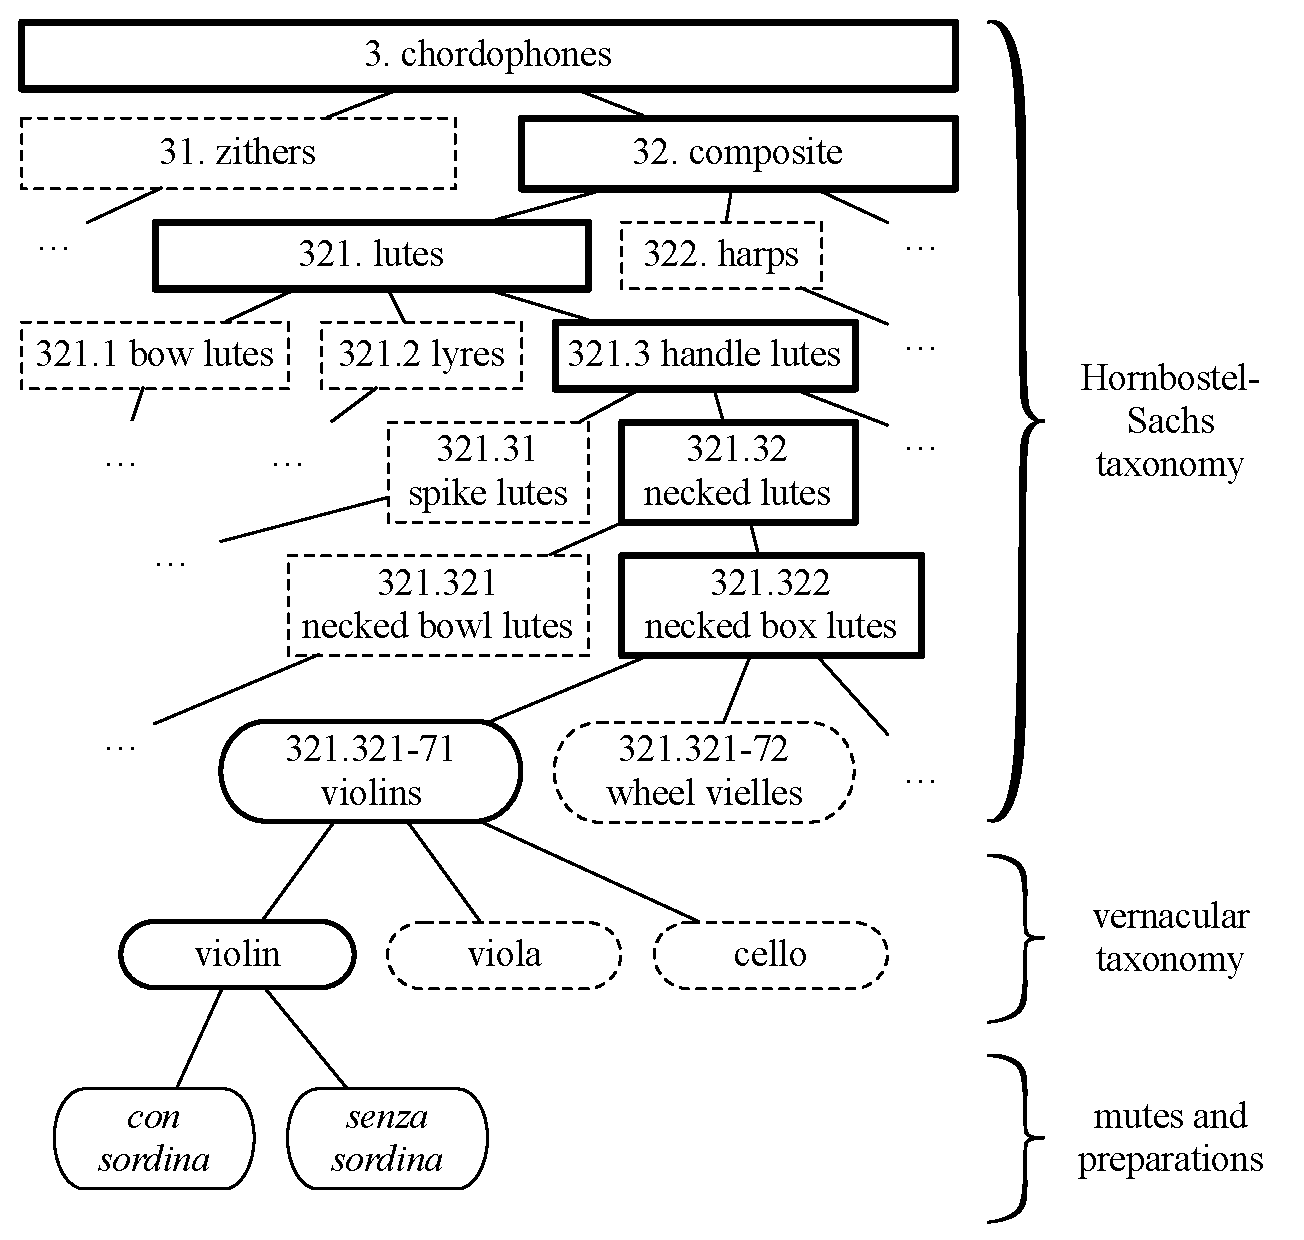
\includegraphics[width=\linewidth]{./figs/dendrograms/instrument-dendrogram.eps}
\caption{Taxonomy of musical instruments.}
\label{fig:instrument-dendrogram}
\end{figure}

Unlike musical instruments, which are approximately amenable to a hierarchical taxonomy of resonating objects, IPTs result from a complex synchronization between multiple gestures, which may involve both hands and arms, as well as diaphragm, vocal tract, and sometimes the whole body.
As a result, there is no immediate way to interface them with H-S, or indeed any tree-like structure \cite{kolozali2011ismir}.
Instead, every playing technique is described by a finite collection of categories, each belonging to a different ``name\-space''; Figure \ref{fig:technique-dendrogram} illustrates such namespaces in the case of the violin.
It therefore appears that, rather than aiming for a mere increase in granularity with respect to H-S, a coherent research program around extended playing techniques should formulate them as belonging to a meronomy, \ie{} a modular entanglement of part-whole relationships, in the fashion of the Visipedia initiative in computer vision \cite{belongie2015pattern}.
In recent years, some publications have attempted to lay the foundations of such a modular approach, with the aim of making H-S relevant to contemporary music creation \cite{magnusson2017jnmr,weisser2011ytm}; yet, such considerations are still in large part speculative, and offer no definitive procedure for evaluating, let alone training, information retrieval systems.

\begin{figure}
\centering
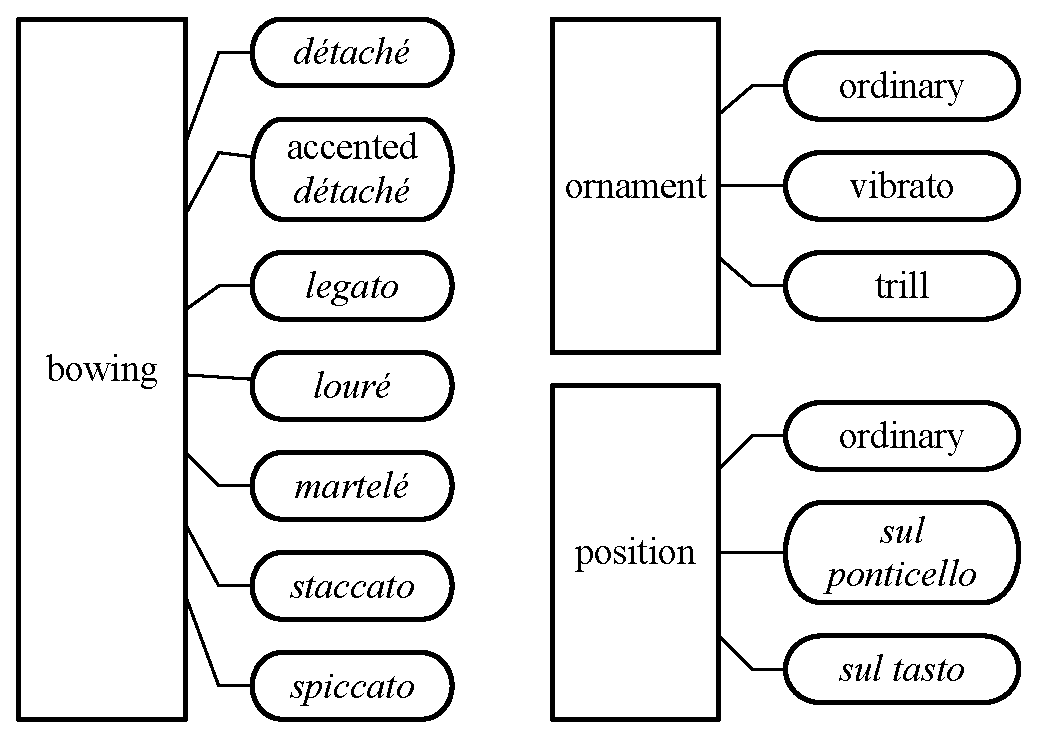
\includegraphics[width=\linewidth]{./figs/dendrograms/technique-dendrogram.eps}
\caption{Namespaces of violin playing techniques.}
\label{fig:technique-dendrogram}
\end{figure}


\subsection{Application setting and evaluation} \label{sec:motivation}

In what follows, we adopt a middle ground position between the two aforementioned approaches: neither a supervised classifier (as in a hierarchical taxonomy), nor a caption generator (as in a meronomy), our system is a query-by-example search engine in a large database of isolated notes.
This system is meant to provide a small number $k$ of nearest neighbors in the dataset of musical instrument samples to any user-defined audio query $\boldsymbol{x}(t)$.
In the context of contemporary music creation, this $\boldsymbol{x}(t)$ may be an instrumental or vocal sketch; a sound event recorded from the environment; a computer-generated waveform; or any mixture of the above \cite{maresz2013cmr}.
Upon inspecting the $k$ nearest neighbors returned by the search engine, the composer may decide to retain one of the retrieved notes, in which case its attributes (pitch and intensity, but also the exact playing technique) are readily available and can be included into the musical score to approximate the query.

Faithfully evaluating such a system is a difficult procedure, and ultimately would rest on its practical usability, as judged by the composers themselves.
Nevertheless, a useful quantitative metric for this task is the precision at $k$ (P@$k$) of the test set with respect to the training set, both under a instrument taxonomy and an IPT taxonomy.
In all subsequent experiments, we report $P@k$ after setting the number of retrieved items to $k=5$.

\subsection{Studio On Line dataset (SOL)}

The Studio On Line dataset (SOL) was recorded at Ircam in 2002 and is freely downloadable as part of the Orchids software for computer-assisted orchestration.\footnote{Link to SOL dataset: \url{http://forumnet.ircam.fr/product/orchids-en/}}
It comprises 16 musical instruments playing $25444$ isolated notes in total.
The distribution of these notes, shown in Figure \ref{fig:instrument-histogram}, spans the full combinatorial diversity of applicable intensities, pitches, preparations (\ie{} mutes), as well as all applicable playing techniques.
The distribution of playing techniques -- whose most common are shown in Figure \ref{fig:technique-histogram} -- is heavy-tailed (average $178$, standard deviation $429$): this is because some playing techniques are shared between many instruments (\eg{} \textit{tremolo}) whereas other are instrument-specific (\eg{} \textit{xylophonic} which is specific to the harp).
The SOL dataset has $143$ IPTs in total, and $469$ applicable instrument-mute-technique triplets.

\begin{figure}[t!]
\centering
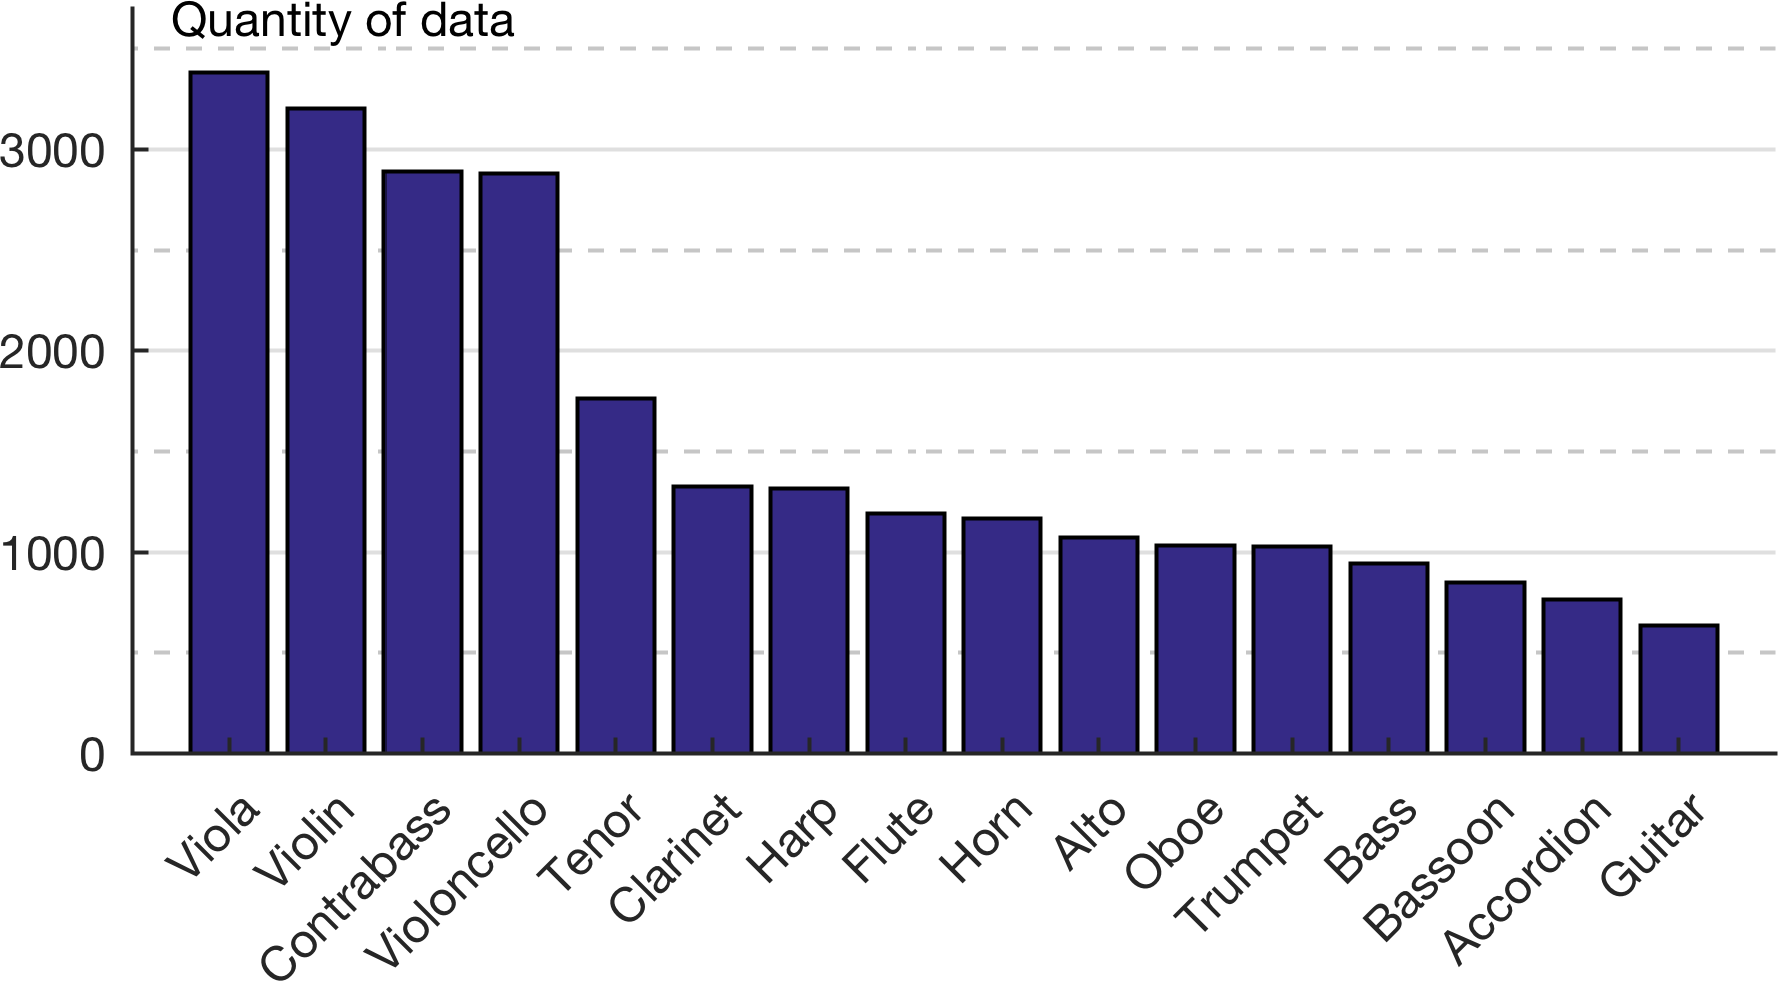
\includegraphics[width=\linewidth]{./figs/histogram/histogram_instruments.png}
\caption{Instruments in the SOL dataset.}
\label{fig:instrument-histogram}
\end{figure}

\begin{figure}[h!]
\centering
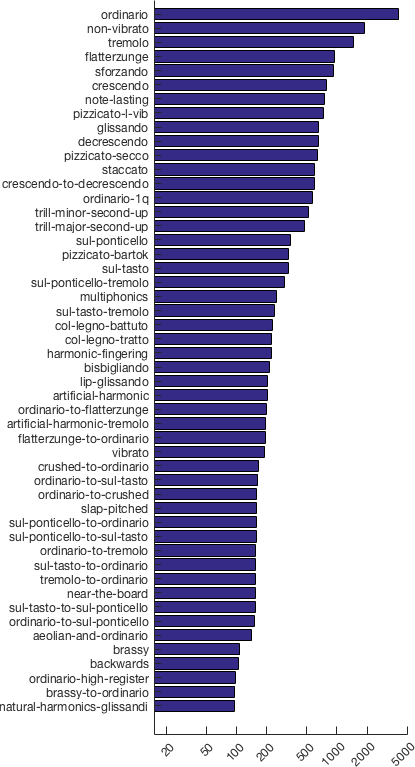
\includegraphics[width=\linewidth]{./figs/histogram/histogram_modes.png}
\caption{Playing techniques in the SOL dataset.}
\label{fig:technique-histogram}
\end{figure}


% Bows and mallets are part of the gesture
% The use of mutes is part of the instrument BUT any gesture while holding the mute (e.g.  trombone) creates a new IPT category that is distinct from ordinary style.

% Out of scope are:
% Variations in articulation: trill, slide. Unlike vibrato, they have a melodic function.
% Variations in: artificial harmonics, subharmonics [ref Mari Kimura],
% Variations in phrasing: arpeggio,
% analog FX


%%%%%%%%%%%%%%%%%%%%%%%%%%%%%%%%%%  METHODS  %%%%%%%%%%%%%%%%%%%%%%%%%%%%%%%%%%%
\section{Methods}

In this section, we describe the scattering transform and supervised metric learning used to implement all query-by-example systems in our benchmark.

\subsection{Scattering transform} % Scattering transform
The scattering transform is a cascade of two wavelet modulus operators:
the first layer extracts the average spectral envelope $\mathbf{S}_1 \boldsymbol{x} (\lambda_1)$ of $\boldsymbol{x}(t)$ at frequencies $\lambda_1$, whereas the second layer $\mathbf{S}_2 \boldsymbol{x} (\lambda_1, \lambda_2)$ extracts amplitude modulations of this spectral envelope at rates $\lambda_2$.
The set of frequencies discretizes the auditory range according to the mel scale, with $Q_1 = 12$ bins per octave at topmost frequencies; whereas rates $\lambda_2$ follow a geometric sequence between $\lambda_1$ and some minimal rate $T^{-1}$, with $Q_2 = 1$ bin per octave.
We refer to \cite{anden2014taslp} for a general introduction to scattering transforms in audio classification, and to \cite{lostanlen2017phd} for a discussion on its application to musical instrument classification in solo recordings, as well as its close connections with STRF. The scattering transform is theoretically suited to model extended playing techniques, since various values of the rate $\lambda_2$ provably characterize some of the most common nonstationarities in sound production, including tremolo, vibrato, and dissonance \cite{anden2012dafx}.
In the following, we denote by $\mathbf{S}\boldsymbol{x}(\lambda)$ the concatenation of all scattering coefficients, whether the generic scattering path $\lambda$ corresponds to a singleton $(\lambda_1)$ or a pair $(\lambda_1,\lambda_2)$.

In order to match a decibel-like perception of loudness, we apply the path-adaptive, quasi-logarithmic compression
\begin{equation}
\widetilde{\mathbf{S}} \boldsymbol{x}_i(\lambda) =
\log \left(
1 + \dfrac{\mathbf{S}\boldsymbol{x}_i(\lambda)}{\varepsilon \times \boldsymbol{\mu}(\lambda)}
\right)
\end{equation}
where $\varepsilon = 10^{-3}$ and $\boldsymbol{\mu}(\lambda)$ is the median value of the scattering coefficient $\mathbf{S}\boldsymbol{x}_i (\lambda)$ for path $\lambda$ across samples $i$.


\subsection{Metric learning} % Large-margin nearest neighbors

%As shown in the experiments described in Section \ref{sec:exp}, it is helpful to consider a supervised projection of the scattering coefficients in order to select among the large dimensionality of the resulting feature space, which axes are relevant for the task at hand.

%One standard approach is the use of the linear discriminant analysis (LDA) that linearly projects ($x \rightarrow L x$) the input data into a features space of $C$-1 dimensions that maximizes the amount of between-class variance relative to the amount of within-class variance. The linear transformation $L$ is chosen to maximize the ratio of between-class to within-class variance, subject to the constraint that $L$ defines a projection matrix.

Linear metric learning algorithms generate a matrix $\mathbf{L}$ such that the Mahalanobis distance
\begin{equation}
\mathrm{D}_\mathbf{L}(\boldsymbol{x}_i, \boldsymbol{x}_j) = (\widetilde{\mathbf{S}}\boldsymbol{x}_i - \widetilde{\mathbf{S}}\boldsymbol{x}_j)^{\top}  \mathbf{L}^{\top} \mathbf{L} (\widetilde{\mathbf{S}}\boldsymbol{x}_i-\widetilde{\mathbf{S}}\boldsymbol{x}_j)
\end{equation}
between all pairs of samples $(\boldsymbol{x}_i, \boldsymbol{x}_j)$ optimizes some objective function.
Observe that the Euclidean distance is a particular case of the equation above, in which case $\mathbf{L}$ boils down to identity.
We refer to \cite{bellet2013survey} for a review of the state of the art.
In particular, the large-margin nearest neighbors (LMNN) algorithm aims at bringing all $k$ nearest neighbors $\boldsymbol{x}_j$ of every $\boldsymbol{x}_i$ closer than the canonical Euclidean distance $\mathrm{D}(\boldsymbol{x}_i, \boldsymbol{x}_j) = \Vert \widetilde{\mathbf{S}}\boldsymbol{x}_i - \widetilde{\mathbf{S}}\boldsymbol{x}_j \Vert$ if $\boldsymbol{x}_i$ and $\boldsymbol{x}_j$ belong to the same class, and further apart otherwise \cite{weinberger2009jmlr}.

As compared to a class-wise generative model (such as Gaussian mixtures), a global linear model ensures some robustness to minor alterations of the taxonomy, which is important in the context of IPT: \eg{} what some instrumentists may call $\emph{slide}$, others will call $\emph{glissando}$.
Furthermore, although one of its major drawback relies on its strong dependency on the Euclidean neighbors to determine intra-class variability \cite{mcfee2010icml}, this drawback is alleviated in the case of a feature space based on scattering transform coefficients, whose Euclidean metric provably approximates the extent of elastic deformation needed to shear $\boldsymbol{x}_i(t)$ into $\boldsymbol{x}_j(t)$ in the time-frequency domain \cite[Theorem 2.16]{mallat2012cpam}.

%%%%%%%%%%%%%%%%%%%%%%%%%%%%%%%%%%%%%%%%%%%%%%%%%%%%%%%%%%%%%%%%%%%%%%%%%%%%%%%%
%%%%%%%%%%%%%%%%%%%%%%%%%%%% EXPERIMENTAL RESULTS %%%%%%%%%%%%%%%%%%%%%%%%%%%%%%
\section{Experimental results} \label{sec:exp}
In this section, we apply the aforementioned methods to instrument and IPT query-by-example retrieval in the Studio On Line (SOL) dataset.

%As explained in Section \ref{sec:motivation}, we formulate here the instrument / playing techniques recognition problem as a query by example one as we are \textit{in fine} interested in an application scenario where the user specify a seed sound, be it played by a musical instrument or not, and the system returns several items from the database that have some level of similarity with the seed.

%Designing such a system would requires the definition of a reference similarity space where the similarity among musical tones is defined perceptually. The acquisition of such reference is out of the scope of this paper and is left for future work. We thus aim here at validating the processing pipeline considered to implement the query by example system. We would like that such architecture is able to effectively rank items of the database according to 1) the partition of the musical instruments and 2) the partition of the playing techniques.


%To evaluate the performance of the alternative implementations of the query by example system, the precision at rank $k$ (p@k) is considered. It is computed as the number of relevant items among the $k$ items retrieved by the system divided by $k$. Revelance here is evaluated as the seed and the retrieved item having the same label in the reference partition. Each item of the database is considered as a seed, and the precision of the system under evaluation is computed for this seed. The precision for this system is the precision averaged over all the seeds.

%When considering a train /test split corpus, the seeds are taken from the test set and  items of the train corpus similar to this seed are retrieved. The precision for this seed is computed among those retrieved items and the precision for the system under evaluation is the precision averaged over all the items of the test set.

%For each sound, some features are computed over a given time frame, ranging from 25 ms. to 1 second. The set of frames is averaged to give one feature vector per sound recording. Unless otherwise stated, discussed results are given for a frame size of 25 ms. \ml{please rephrase : While considering a short frame size increases the number of frames and thus stabilizes the averaging}, it reduces the ability of the feature to model long time range modulations.


\subsection{Evaluation of instrument recognition}

In the task of instrument recognition, each of the $k$ elements $\boldsymbol{x}_j$ returned by the system is considered relevant to the query $\boldsymbol{x}_i$ if and only if $\boldsymbol{x}_i$ and $\boldsymbol{x}_j$ correspond to the same instrument, regardless of pitch, intensity, mute, and playing technique.

We compare scattering features to a baseline of mel-frequency cepstral coefficients (MFCC), corresponding to the $13$ lowest quefrencies after applying a discrete cosine transform (DCT) on the logarithm of the $40$-band mel-frequency spectrum.
In addition, we vary the maximum time scale $T$ of amplitude modulation between \SI{25}{\milli\second} and  \SI{1}{\second}.
In the case of MFCC, $T=\SI{25}{\milli\second}$ corresponds to the inverse of the lowest audible frequency ($T^{-1}=\SI{40}{\Hz}$).
Therefore, increasing the frame duration $T$ has no effect on the value of MFCC, because the mel-spectrogram is equivalent to a local averaging of the wavelet scalogram at the time scale $T$, leaving unchanged the global averaging of $\mathbf{S}\boldsymbol{x}(\lambda)$ at the time scale of whole musical notes \cite{anden2012dafx}.

Figure \ref{fig:results} (left) summarizes our results.
We find that MFCC reach a relatively high P@5 of $89\%$.
Keeping all $40$ quefrencies rather than the lowest $13$ brings the P@5 down to $84\%$, because the highest quefrencies are the most affected by some spurious factors of intra-class variability, namely pitch and spectral flatness \cite{lostanlen2017phd}.

At the smallest time scale $T=\SI{25}{\milli\second}$, the scattering transform reaches a P@5 of $89\%$, thus matching exactly the performance of MFCC.
This is because the relatively few second-order scattering coefficients whose rate $\lambda_2$ exceeds $\SI{40}{\Hz}$ have a negligible effect on Euclidean distances, as they carry very little energy \cite{anden2014taslp}.
Moreover, disabling median renormalization -- \ie{} setting $\boldsymbol{\mu}(\lambda) = 1$ for all scattering paths $\lambda$ -- degrades P@5 down to $84\%$, while disabling logarithmic compression altogether -- \ie{} the limit case $\varepsilon \rightarrow \infty$ -- degrades it to $76\%$.
These results are consistent with another publication \cite{lostanlen2018eurasip}, which applies scattering transform to a query-by-example retrieval task among environmental acoustic scenes.

On one hand, replacing the canonical Euclidean distance by a Mahalanobis distance learned by the LMNN algorithm marginally improve P@5 in the case of the MFCC baseline, from $89.3\%$ to $90.0\%$.
On the other hand, applying LMNN on scattering features strongly enhances their performance with respect to the Euclidean distance, from $89.1\%$ to $98.0\%$.

The gain in precision afforded by scattering coefficients over MFCC could simply be caused by a higher number of dimensions.
To refute this hypothesis, we supplement the $13$ coefficients resulting from a global averaging at the time scale of full musical notes by higher-order summary statistics, namely polynomial features of degrees $2$ and $3$.
Instrument retrieval in the resulting feature space, whose dimension ($494$) is comparable to the number of scattering coefficients, has a P@5 of $91\%$, \ie{} slightly above the baseline.
Therefore, it is more likely the multiresolution structure of scattering coefficients, rather than its dimensionality, that causes a strong boost in performance.

Lastly, increasing $T$ from $\SI{25}{\milli\second}$ up to $\SI{1}{\second}$ -- that is, including all amplitude modulations between $\SI{1}{\Hz}$ and $\SI{40}{\Hz}$ -- brings LMNN to a near-perfect P@5 of $99.71\%$.
Not only does this result confirm that well-established methods in audio signal processing (here, wavelet scattering and metric learning) are sufficient to retrieve the instrument from a single ordinary note; it also demonstrates that the results remain excellent despite large intra-class variability within instruments: in pitch and intensity, but also in the usage of mutes and extended IPTs.
In other words, the monophonic recognition of Western instruments is, all things considered, a solved problem indeed.

\begin{figure}
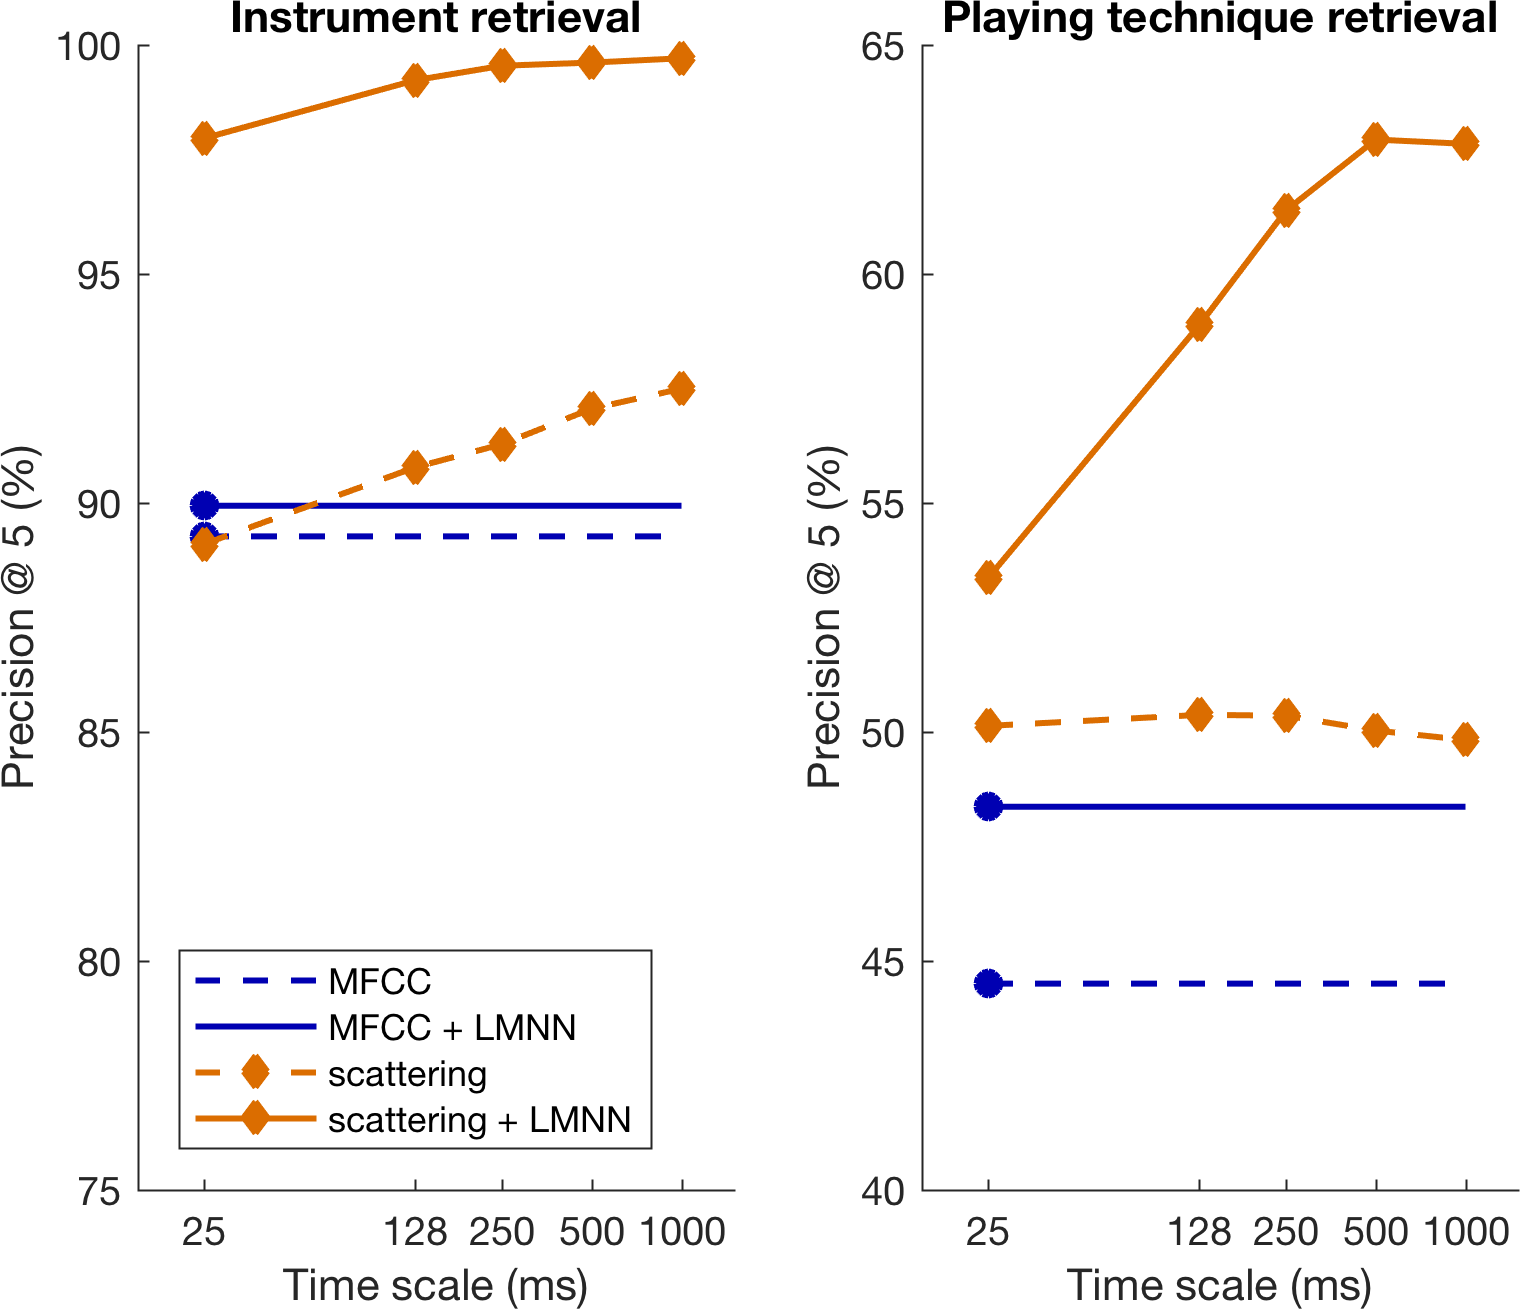
\includegraphics[width=\linewidth,keepaspectratio]{./figs/results/results.png}
\caption{Summary of results on the SOL dataset.}
\label{fig:results}
\end{figure}

\subsection{Evaluation of playing technique recognition}

The situation is different when considering IPT, rather than instrument, as reference for evaluating the reference of the query-by-example search engine.
The MFCC baseline has a relatively low P@5 of $44.5\%$, which indicates that a coarse description of the short-term spectral envelope is rarely ever sufficient to model acoustic similarity in IPT.
Perhaps more surprisingly, we find that only the system combining all presented improvements, \ie{} log-scattering coefficients with median renormalization, $T=\SI{500}{\milli\second}$, and LMNN, strongly outperforms the MFCC baseline, with a state-of-the-art P@5 of $63.0\%$.
Indeed, an ablation study of that system reveals that, all other things being equal: reducing $T$ to $\SI{25}{\milli\second}$ brings the P@5 to $53.3\%$; disabling LMNN, $50.0\%$; and replacing scattering coefficients by MFCC, to $48.4\%$.

What stems from these observations is that, unlike instrument similarity, IPT similarity results from long-range temporal dependencies in the audio signal.
In addition, the dissimilarity between two different playing techniques is not a matter of elastic deformation in the time-frequency domain -- as approximated by Euclidean distance in the feature space of scattering coefficients -- but also involves an adaptive process which combines the saliences of various acoustic frequencies and modulation rates in several nonuniform ways, thus producing a metric that favors certain factors of acoustic variability while mitigating others.

%As expected, considering the playing technique partition as a reference gives a harder task to perform as the  MFCC baseline achieves a p@5 of $45\%$ and the scattering a p@5 of $50\%$.
%When considering a frame size of 25 ms., the LMNN projection gives an equivalent

%\subsection{Pitch-adaptive metric learning}
%A well-known rule of thumb in psychoacoustics states that the ``bandwidth for timbre invariance'', \ie{} the musical interval beyond which two notes are judged dissimilar, is of the order of one octave for untrained listeners \cite{handel2001musicperception} and up to $2.5$ octaves for trained listeners \cite{steele2006musicperception}.

%Again, enlarging the frame size do not influence the performance of the MFCC baseline, see Figure \ref{fig:results}(right). More surprisingly, the performance of the scattering features stalls with respect of the frame size. In increase would have been expected, since many playing techniques involves long term modulation of energy through frequency bands which are expected to be nicely captured by the scattering features.

%It is only when considering the LMNN projection that the p@5 strongly increases with respect to the frame size. We believe that the fact that the system benefit from a richer input only if a supervised projection is considered is due to the need to select \textit{a priori} among the large range of modulations modeled by the scattering features the ones that are relevant for the task at hand.


%%%%%%%%%%%%%%%%%%%%%%%%%%%%%%%%%%%%%%%%%%%%%%%%%%%%%%%%%%%%%%%%%%%%%%%%%%%%%%%%
%%%%%%%%%%%%%%%%%%%%%%%%%%%%%%%%%  CONCLUSION  %%%%%%%%%%%%%%%%%%%%%%%%%%%%%%%%%
\section{Conclusion}

Whereas the MIR literature abounds on the topic of musical instrument recognition in so-called ``ordinary'' isolated notes and solo performances, little is known about the problem of retrieving the instrumental playing technique (IPT) of an audio query within a fine-grained taxonomy.
Yet, the knowledge of IPT is a precious source of music information, not only to characterize the physical interaction between player and instrument, but also in the realm of contemporary music creation.
In all likelihood, it also bears an interest for organizing digital libraries, as a mid-level descriptor of musical style.
To the best of our knowledge, this paper is the first in benchmarking query-by-example MIR systems according to a large-vocabulary IPT reference (143 classes) instead of an instrument reference.
We find that this new task is considerably more challenging than musical instrument recognition, as it amounts to characterizing spectrotemporal patterns at various scales and rates and comparing them in a highly non-Euclidean way.
Although the combination of methods presented here -- wavelet scattering and large-margin nearest neighbors -- outperforms the MFCC baseline (even at comparable dimensionalities and number of learnable parameters), its accuracy on the SOL dataset certainly leaves some room for future improvements.

The evaluation methodology presented here uses ground truth IPT labels to quantify the relevance of returned items.
Despite the advantage of unequivocality, it might be too harsh to reflect practical use.
Indeed, as it is often the case in MIR, some pairs of labels are subjectively more similar than others: \eg{} \emph{slide} is evidently closer to \emph{glissando} than to \emph{pizzicato-bartok}.
The collection of subjective ratings of IPT similarity, and its comparison with automated ratings, is left as future work.
%employs a $0-1$ loss to discriminate IPTs.

%playing technique is important to fully describe the interaction between a performer and a instrument.

%playing technique modeling

%need to capture long term modulations

%scattering useful for this end

%benchmark results demonstrate the need to have a supervised step to specialize the representation

%The results described in this paper validate the processing pipeline on the reference partitions of instruments and playing techniques. Future work will focus on the definition of a reference similarity among couples of instruments and playing techniques that is defined perceptually and the evaluation of the proposed processing pipeline against this perceptually defined reference.

%Every quest for information is also a quest for invariance. [...]
% We have formulated the problem as query-by-example browsing. Another possible formulation would be textual description.

% Our main finding is that mel-frequency cepstral coefficients (MFCC), although highly informative for musical instrument recognition in so-called ``ordinary'' notes, fail to discriminate extended instrumental techniques for at least three reasons.
% First, they summarize spectral envelope without retaining its amplitude modulations.
% Secondly, the frame rate at which they are computed ($T=\SI{25}{\milli\second}$ or so) is short enough to assume local stationarity, but not long enough to encompass all informative local correlations.
% Thirdly, the discrete cosine transform (DCT) over mel frequencies does not, contrary to a widespread belief, make them invariant to the frequency transposition of complex sounds.
% To address each of these shortcomings, we propose a simple pipeline of three elements: a time scattering transform; an unsupervised renormalization procedure; and a supervised metric learning over frequencies and modulation rates with large-margin nearest neighbors (LMNN).

% Matching a reference similarity is left as future work.

%\section{Acknowledgments}
% The authors wish to thank Andrew Farnsworth and (?) for fruitful discussions on Visipedia.
% TICEL people.
% Catherine Krocker for helpful suggestions on the title of this article.



% For bibtex users:
\bibliography{lostanlenPlayingTechniques}

\end{document}
